\documentclass[preview, border=2mm]{standalone}

\renewcommand{\rmdefault}{\sfdefault}	% sets main text to sans-serif
\usepackage{mathastext}				% makes math use the text font

\usepackage{amsmath}

\usepackage{tikz}

\begin{document}

\vspace*{\fill}

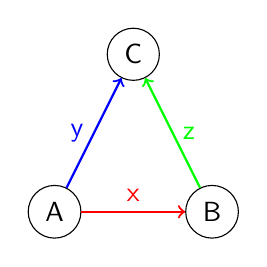
\begin{tikzpicture}
    % Define nodes
    \node[circle, draw] (A) at (0,0) {$A$};
    \node[circle, draw] (B) at (2,0) {$B$};
    \node[circle, draw] (C) at (1,2) {$C$};

    % Define edges with labels
    \draw[->, red, thick] (A) -- node [midway, above] {$x$} (B);
    \draw[->, blue, thick] (A) -- node [midway, left] {$y$} (C);
    \draw[->, green, thick] (B) -- node [midway, right] {$z$} (C);
\end{tikzpicture}

\vspace*{\fill}

\end{document}
